% CS604 final report (Team 06), written with the CVPR 2026 author kit:
% https://github.com/cvpr-org/author-kit (tag CVPR2026-v1(latex)).
% Compile with pdfLaTeX + BibTeX (e.g. on Overleaf): pdflatex -> bibtex -> pdflatex -> pdflatex.

\documentclass[10pt,twocolumn,letterpaper]{article}

%%%%%%%%% PAPER TYPE
% Camera-ready layout (no review ruler, authors shown), with page numbers for the course submission.
\usepackage[pagenumbers]{cvpr}

% Import additional packages in the preamble file, before hyperref
%% This file contains a number of tweaks that are typically applied to the main document.
%% They are not enabled by default, but can be enabled by uncommenting the relevant lines.

%%
%% Inline annotations; for predefined colors, refer to "dvipsnames" in the xcolor package:
%% https://tinyurl.com/overleaf-colors
%%
\newcommand{\red}[1]{{\color{red}#1}}
\newcommand{\todo}[1]{{\color{red}#1}}
\newcommand{\TODO}[1]{\textbf{\color{red}[TODO: #1]}}
%%
%% disable for camera ready / submission by uncommenting these lines  
%%
% \renewcommand{\TODO}[1]{}
% \renewcommand{\todo}[1]{#1}

%%
%% work harder in optimizing text layout. Typically shrinks text by 1/6 of page, enable
%% it at the very end of the writing process, when you are just above the page limit
%%
% \usepackage{microtype}

%%
%% fine-tune paragraph spacing
%%
% \renewcommand{\paragraph}[1]{\vspace{.5em}\noindent\textbf{#1.}}

%%
%% globally adjusts space between figure and caption
%%
% \setlength{\abovecaptionskip}{.5em}


%%
%% Allows "the use of \paper to refer to the project name"
%% with automatic management of space at the end of the word
%%
% \usepackage{xspace}
% \newcommand{\paper}{ProjectName\xspace}

%%
%% Commonly used math definitions
%%
% \DeclareMathOperator*{\argmin}{arg\,min}
% \DeclareMathOperator*{\argmax}{arg\,max}

%%
%% Tigthen underline
%%
% \usepackage{soul}
% \setuldepth{foobar}

%%
%% CS604 report additions
%%
\usepackage{microtype}   % better line breaking in the two-column layout
\usepackage{multirow}
\newcommand{\run}[1]{\texttt{#1}}  % run identifiers (escape underscores as \_)
\newcommand{\minus}{\ensuremath{-}}

\definecolor{cvprblue}{rgb}{0.21,0.49,0.74}
\usepackage[pagebackref,breaklinks,colorlinks,allcolors=cvprblue]{hyperref}

%%%%%%%%% PAPER ID
\def\paperID{06} % course team number; not a CVPR paper ID
\def\confName{CVPR}
\def\confYear{2026}

%%%%%%%%% TITLE
\title{Prototype-Initialized Adaptation of ViT-B/16 for 10,000-Class\\Fine-Grained Classification under a Fixed Compute Budget}

%%%%%%%%% AUTHORS
\author{\todo{Member 1 (student ID)} \qquad \todo{Member 2 (student ID)} \qquad \todo{Member 3 (student ID)}\\
CS604 Team 06, Singapore Management University\\
{\tt\small \todo{email addresses}}
}

\begin{document}
\maketitle
\begin{abstract}
We adapt a ViT-B/16 pretrained on ImageNet-21k and fine-tuned on ImageNet-1k to an anonymized fine-grained benchmark with 10,000 classes and only 45 labeled images per class, under a budget of 2 hours on 48\,GB of GPU memory per training run.
We compare full fine-tuning with parameter-efficient adaptation (LoRA and AdaptFormer) and find that the most important design decision is how the new 10,000-way classifier head is initialized.
Initializing it with a linear probe fitted on frozen training features, a common way to avoid a random head, consistently hurts.
Imprinting L2-normalized class-mean prototypes instead improves holdout accuracy by about 2.5 points for both full fine-tuning and LoRA, and the validation accuracy of our final model by 3.1 points under otherwise identical settings.
Together with training on all images and horizontal-flip test-time augmentation, our final full fine-tuning model reaches 76.22\% top-1 accuracy on the CodaBench validation set (reference: 70.8\%) using 1.03 GPU-hours on one A100.
Our best parameter-efficient model applies LoRA to every linear layer of the backbone, trains 1.375\% of its parameters, and reaches 71.90\% (reference LoRA: 68.3\%) with no inference overhead after the low-rank updates are merged.
\end{abstract}

\section{Introduction}
\label{sec:intro}

Large pretrained Vision Transformers~\cite{dosovitskiy2021vit,steiner2022augreg} are rarely trained from scratch; they are adapted to new tasks, either by fine-tuning all weights or by training a small set of added parameters~\cite{houlsby2019adapter,hu2022lora,chen2022adaptformer}.
In this project we adapt ViT-B/16 to an anonymized fine-grained classification benchmark with 10,000 classes.
The training split has 450,000 images, exactly 45 per class; the validation split (50,000 images, 5 per class) and the test split (100,000 images, 10 per class) have hidden labels and are scored on CodaBench.
Each training run may use at most 2 hours on 48\,GB of GPU memory (96\,GB$\cdot$h), and every method is reported with four metrics: top-1 accuracy, trainable parameters, inference latency and training GPU-hours.

This setting differs from typical transfer-learning benchmarks in two ways.
First, the classifier head is large and data-starved.
A $10{,}000 \times 768$ linear head has 7.69M parameters: 9.0\% of the 85.8M-parameter backbone and 26$\times$ more than a rank-8 LoRA on the attention projections.
Yet each of its rows is trained from only 43--45 images.
Second, the budget is tight.
One epoch of full fine-tuning takes about 6.5 minutes on an A100, so only about eight epochs fit into a run.

These constraints raise three practical questions.
(1)~How should the new head be initialized?
(2)~Where should a parameter-efficient method spend its capacity?
(3)~How should a fixed budget be split between epochs, data and test-time computation?
We answer them with 17 controlled runs, each changing one setting at a time.
We select models on a local holdout split that agrees with the CodaBench validation score to within 0.3 points.
Our contributions are:
\begin{itemize}[leftmargin=*,itemsep=1pt,topsep=2pt]
    \item \textbf{Prototype head initialization.} The common linear-probe (LP) head, which LP-FT~\cite{kumar2022lpft} fits on frozen features before fine-tuning, is harmful in this regime. Imprinting class-mean prototypes~\cite{qi2018imprinted} instead improves accuracy by 2.5--3.1 points for both full fine-tuning and LoRA. Loss curves suggest why (\cref{sec:ablation-head}).
    \item \textbf{An analysis of parameter-efficient adaptation under a budget.} Capacity matters more than the learning rate. LoRA on all linear layers (1.375\% of the backbone) beats LoRA on the attention projections alone by 0.88 points and reaches 98\% of full fine-tuning accuracy under the same settings. Merged LoRA adds no latency, whereas AdaptFormer adds about 35\%. Parameter-efficient training was \emph{not} faster or lighter in memory than full fine-tuning here.
    \item \textbf{A budget-aware recipe with complete accounting.} We report accuracy, trainable parameters, latency, GPU-hours and peak memory for every run. Our final models reach 76.22\% (full fine-tuning, $+$5.4 over the reference) and 71.90\% (LoRA, $+$3.6 over the reference LoRA) on the CodaBench validation set.
\end{itemize}

\section{Related Work}
\label{sec:related}

\paragraph{Vision Transformers and transfer learning.}
ViT~\cite{dosovitskiy2021vit} applies a Transformer~\cite{vaswani2017attention} to a sequence of $16 \times 16$ image patches.
Supervised pretraining on ImageNet-21k~\cite{deng2009imagenet} with strong augmentation and regularization (AugReg~\cite{steiner2022augreg}) produces backbones that transfer well.
We use the AugReg ViT-B/16 checkpoint from timm~\cite{wightman2019timm} that was further fine-tuned on ImageNet-1k.
Better ImageNet models also transfer better, under both linear evaluation and fine-tuning~\cite{kornblith2019better}.
Standard fine-tuning recipes use AdamW~\cite{loshchilov2019adamw}, warmup with cosine decay~\cite{loshchilov2017sgdr}, label smoothing~\cite{szegedy2016rethinking}, stochastic depth~\cite{huang2016stochastic} and layer-wise learning-rate decay~\cite{bao2022beit}; our full fine-tuning baseline follows this practice.

\paragraph{Parameter-efficient fine-tuning (PEFT).}
Adapters insert small bottleneck MLPs into every Transformer block~\cite{houlsby2019adapter}.
AdaptFormer~\cite{chen2022adaptformer} instead adds a scaled bottleneck branch \emph{in parallel} to the MLP of each ViT block.
LoRA~\cite{hu2022lora} learns a low-rank update $\Delta W = BA$ to frozen weight matrices, which can be merged into the weights after training.
VPT~\cite{jia2022vpt} prepends learnable prompt tokens, and BitFit~\cite{benzaken2022bitfit} trains only the bias terms.
We implement LoRA with the PEFT library~\cite{mangrulkar2022peft} and compare it with AdaptFormer.

\paragraph{Initializing the classifier head.}
When a pretrained model is transferred to new classes, the head is usually re-initialized; ViT zero-initializes it~\cite{dosovitskiy2021vit}.
LP-FT~\cite{kumar2022lpft} argues that a randomly initialized head distorts pretrained features during fine-tuning.
It therefore first fits a linear probe on frozen features and then fine-tunes everything.
Prototype-based classifiers represent each class by the mean embedding of its examples, as in prototypical networks~\cite{snell2017prototypical}.
Such normalized class means can be \emph{imprinted} directly as the weights of a cosine classifier~\cite{qi2018imprinted}.
Our prototype head is an imprinted cosine classifier with a fitted temperature.
We compare it with random and linear-probe initialization in a regime that is many-way (10,000 classes) and few-shot per class (45 images), with a short training budget.

\section{Method}
\label{sec:method}

\begin{figure*}[t]
  \centering
  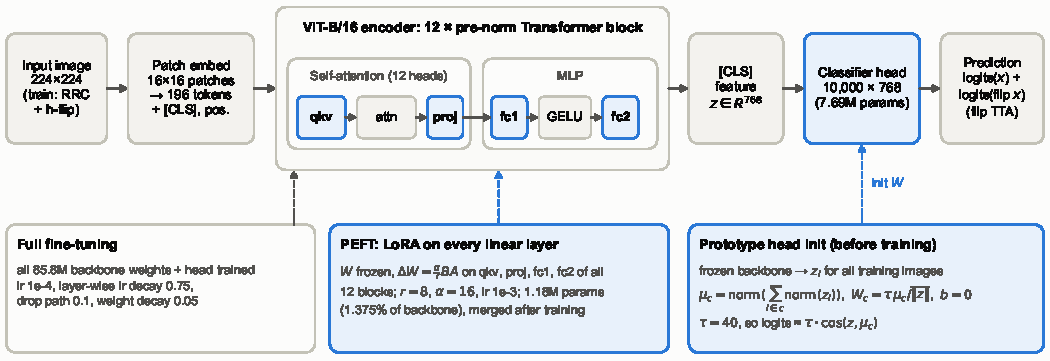
\includegraphics[width=\textwidth]{figures/fig0_framework.pdf}
  \caption{\textbf{Overview of our pipeline.}
  A ViT-B/16 backbone is adapted either by full fine-tuning or by LoRA on every linear layer (blue modules: qkv, proj, fc1, fc2 in all 12 blocks).
  Before training, the 10,000-way head is initialized by imprinting L2-normalized class-mean features (prototypes) with temperature $\tau$.
  At test time, the logits of the image and of its horizontal flip are summed.
  All runs use AdamW with warmup and cosine decay, bf16 and batch size 256, within a budget of 96\,GB$\cdot$h (1.2\,h on one A100-80GB).}
  \label{fig:framework}
\end{figure*}

\Cref{fig:framework} summarizes the pipeline.
Let $f_\theta$ map an image $x$ to its final-layer \texttt{[CLS]} feature $z = f_\theta(x) \in \mathbb{R}^{768}$, and let $h(z) = Wz + b$ with $W \in \mathbb{R}^{10000 \times 768}$ be the new classifier head.

\subsection{Backbone, budget and full fine-tuning}
\label{sec:budget}

\paragraph{Backbone.}
We use the timm~\cite{wightman2019timm} checkpoint \nolinkurl{vit_base_patch16_224.augreg2_in21k_ft_in1k}.
It is ViT-B/16 pretrained on ImageNet-21k with AugReg~\cite{steiner2022augreg} and fine-tuned on ImageNet-1k.
The backbone has 85,798,656 parameters; the 1,000-class head is replaced by a new 10,000-class head with 7,690,000 parameters.

\paragraph{Compute budget.}
The project allows 2\,h$\times$48\,GB $=$ 96\,GB$\cdot$h per training run ($\pm$10\%).
We convert this by the memory of the card we use: 1.2\,h on an 80\,GB A100.
Our clock counts everything that uses the GPU for training: head initialization (including feature extraction), all optimizer steps, and the holdout evaluation after every epoch.
It excludes unpacking the data, writing checkpoints and the final predictions.
After timing training steps 20--120, the cosine schedule is compressed if the planned number of epochs would exceed 97\% of the budget, and training stops at 1.05$\times$ the budget.
Every run reported here finished within 1.06 GPU-hours.

\paragraph{Full fine-tuning.}
All backbone and head weights are trained with AdamW~\cite{loshchilov2019adamw} at learning rate $10^{-4}$ and weight decay 0.05 (none on biases, normalization parameters, the class token and position embeddings).
We use layer-wise learning-rate decay of 0.75~\cite{bao2022beit} and drop path 0.1~\cite{huang2016stochastic}.
The learning rate warms up linearly (one epoch for runs of 6 or more epochs, 0.3 epochs for 3-epoch runs) and then follows a cosine decay to zero~\cite{loshchilov2017sgdr}.
Other settings are batch size 256, bf16 mixed precision, gradient clipping at norm 1, and label smoothing 0.1~\cite{szegedy2016rethinking}.
Training augmentation is RandomResizedCrop (scale 0.25--1) plus horizontal flip.
For evaluation, images are resized to 248 pixels and center-cropped to 224.

\subsection{Parameter-efficient adaptation}
\label{sec:peft}

\paragraph{LoRA.}
For a frozen linear layer $W_0 \in \mathbb{R}^{d_\text{out} \times d_\text{in}}$, LoRA~\cite{hu2022lora} computes
\begin{equation}
  y = W_0 x + \tfrac{\alpha}{r} B A x,
  \label{eq:lora}
\end{equation}
where $A \in \mathbb{R}^{r \times d_\text{in}}$ and $B \in \mathbb{R}^{d_\text{out} \times r}$ are trainable.
$B$ is initialized to zero, so training starts exactly from the pretrained model.
We use $r = 8$ and $\alpha = 16$.
timm fuses the query, key and value projections into a single \texttt{qkv} layer.
LoRA on \texttt{qkv} therefore adapts all three projections, with the same parameter count (294,912, 0.344\% of the backbone) as LoRA on separate query and value projections.
Our final PEFT variant applies LoRA to all four linear layers of every block (\texttt{qkv}, \texttt{proj}, \texttt{fc1}, \texttt{fc2}), for 1,179,648 parameters (1.375\%).
The LoRA weights and the head use learning rate $10^{-3}$ and weight decay $10^{-4}$, with no LoRA dropout.
After training, $\tfrac{\alpha}{r}BA$ is merged into $W_0$, so inference uses exactly the base architecture.

\paragraph{AdaptFormer.}
Following~\cite{chen2022adaptformer}, each block gains a bottleneck branch in parallel to its MLP:
\begin{equation}
  x_{l+1} = x' + \mathrm{MLP}(\mathrm{LN}(x')) + s \cdot W_\text{up}\,\mathrm{ReLU}(W_\text{down} x'),
  \label{eq:adaptformer}
\end{equation}
where $x'$ is the output of the attention sub-block.
We use bottleneck width 64, scale $s = 0.1$, dropout 0.1 and a zero-initialized $W_\text{up}$, for 1,189,632 parameters (1.387\%).
Unlike LoRA, the branch cannot be merged into the backbone.

In all PEFT runs the head is also trained.
Because the head alone has 7.69M parameters, we report trainable parameters both excluding it (the convention of the project's 0.34\% LoRA reference) and including it.

\subsection{Initializing the 10,000-way head}
\label{sec:head-init}

The head is the largest new component, and each of its rows sees at most 45 images.
A random head produces near-uniform logits (initial loss $\approx \ln 10000 = 9.2$), and the backbone receives large, noisy gradients from it early in training.
We compare three initializations.

\paragraph{Random.} timm's default initialization of a new linear layer.

\paragraph{Prototype (imprinted) head.}
With the frozen pretrained backbone, we extract features $z_i$ for all training images once.
We then imprint L2-normalized class means~\cite{snell2017prototypical,qi2018imprinted}:
\begin{equation}
  \mu_c = \frac{\sum_{i:\,y_i=c} \hat z_i}{\big\|\sum_{i:\,y_i=c} \hat z_i\big\|}, \quad
  W_c = \frac{\tau}{\overline{\|z\|}}\, \mu_c, \quad b_c = 0,
  \label{eq:proto}
\end{equation}
where $\hat z_i = z_i / \|z_i\|$ and $\overline{\|z\|}$ is the mean feature norm, so that logits are approximately $\tau \cos(z, \mu_c)$.
The temperature $\tau$ is chosen from $\{5, 10, 15, 20, 30, 40, 60, 80\}$ by the cross-entropy on 10,000 training features, which selects $\tau = 40$.
This head alone, with zero trainable parameters, reaches 44.0\% holdout accuracy.
Feature extraction takes 6--7 minutes on an A100, and this time is counted in every run's GPU-hours.

\paragraph{Linear-probe (LP) head.}
Starting from the prototype head, we train $(W, b)$ on the cached frozen features for 10 epochs.
We use AdamW (learning rate $10^{-3}$, weight decay $10^{-4}$), batch size 4,096, cosine decay and label smoothing 0.1.
This reaches 62.1\% holdout accuracy in a few seconds and corresponds to the first stage of LP-FT~\cite{kumar2022lpft}.
It was our initial design, chosen to avoid feature distortion from a random head.
\Cref{sec:ablation-head} shows that it is the worst of the three choices.

\subsection{Test-time augmentation}
Following common practice~\cite{krizhevsky2012imagenet}, we sum the logits of an image and its horizontal flip.
This doubles inference cost and is applied only where stated.

\section{Experiments}
\label{sec:experiments}

\subsection{Setup}
\label{sec:setup}

\paragraph{Data and protocol.}
Validation and test labels are hidden, so we hold out 2 images per class from the training split (20,000 images, fixed seed).
We use this holdout for model selection and ablations, and train on the remaining 43 images per class.
Final models are retrained on all 45 images per class.
Validation and test images are used only to produce submission files.
CodaBench reports top-1 accuracy.
Because the validation set is balanced (5 images per class), top-1 accuracy equals the average per-class accuracy.
Our holdout tracks the server closely: 72.31\% \vs 72.57\% for full fine-tuning and 71.98\% \vs 71.90\% for LoRA.
Differences below about 0.3 points are within holdout noise.
All runs use one seed.

\paragraph{Metrics.}
Latency is the mean time of 100 forward passes of a random $224 \times 224$ input at batch size 1, after 10 warm-up passes, with bf16 autocast on an A100.
Throughput is measured at batch size 256.
Repeated measurements of the same architecture vary by about $\pm$0.4\,ms.
GPU-hours are taken from the clock described in \cref{sec:budget}.
Peak VRAM is the maximum memory allocated by PyTorch during training; the memory reserved by PyTorch is 0.2--1.4\,GB higher (20.1\,GB for the final model).
The appendix contains the supporting material:
\begin{itemize}[leftmargin=*,itemsep=0pt,topsep=2pt]
    \item training-log excerpts with time and VRAM (\cref{sec:logs});
    \item all 17 runs (\cref{tab:all-runs});
    \item the full hyperparameters (\cref{tab:hparams}).
\end{itemize}

\paragraph{Hardware and software.}
All runs use one NVIDIA A100-SXM4-80GB with 12 CPU cores, except one ablation batch (random and prototype heads for LoRA in \cref{tab:head}), which ran on an RTX PRO 6000 Blackwell.
Repeating its prototype run on the A100 gave 71.98\% \vs 72.00\%, so accuracies are comparable across the two GPUs; speeds and latencies are not.
Software, as logged for our last two batches, which include all final models: PyTorch 2.11.0 (CUDA 13.0), timm 1.0.30 and PEFT 0.21.1. Earlier runs used the then-current releases, which were not logged.

\subsection{Reproducing the reference baselines}

\begin{table}[t]
  \centering
  \footnotesize
  \setlength{\tabcolsep}{4pt}
  \begin{tabular}{@{}lccc@{}}
    \toprule
    Method & Trainable & Reference & Ours \\
    \midrule
    Zero-shot, initialized head & 0\% & 43.7 & 43.95 \\
    Full fine-tuning & 100\% & 70.8 & 70.88 \\
    LoRA ($r=8$) & 0.34\% & 68.3 & 68.57 \\
    \bottomrule
  \end{tabular}
  \caption{\textbf{Reproducing the reference results} from the project description (top-1, \%).
  Ours: holdout accuracy of 3-epoch runs (0.40--0.45 GPU-h) with the linear-probe head; for zero-shot, the prototype head without training.}
  \label{tab:baselines}
\end{table}

Before changing anything, we checked our pipeline against the three reference results in the project description.
Short 3-epoch runs reproduce all three within 0.3 points (\cref{tab:baselines}).
This confirms the data pipeline, the evaluation and our reading of the trainable-parameter convention.

\subsection{Main results}
\label{sec:main}

\begin{table*}[t]
  \centering
  \footnotesize
  \setlength{\tabcolsep}{4pt}
  \begin{tabular}{@{}llcrrrrrrrrr@{}}
    \toprule
    & & & \multicolumn{2}{c}{Trainable params} & \multicolumn{3}{c}{Top-1 accuracy (\%)} & \multicolumn{2}{c}{Inference} & \multicolumn{2}{c}{Training} \\
    \cmidrule(lr){4-5} \cmidrule(lr){6-8} \cmidrule(lr){9-10} \cmidrule(l){11-12}
    Method & Head init & Ep. & Backbone & Head & Holdout & Val & Test & ms (bs 1) & img/s & GPU-h & GB \\
    \midrule
    Zero-shot & prototype & 0 & 0 & 0 & 43.95 & -- & -- & 7.55 & 3,832 & 0.11 & 3.9 \\
    Linear probe & LP & -- & 0 & 7.69M & 62.07 & -- & -- & -- & -- & $\approx$0.11 & -- \\
    \midrule
    Full fine-tuning & LP & 8 & 85.80M (100\%) & 7.69M & 72.31 & 72.57 & -- & 7.35 & 3,864 & 1.03 & 18.9 \\
    \textbf{Full fine-tuning (final)}$^\dagger$ & prototype & 8 & 85.80M (100\%) & 7.69M & -- & \textbf{76.22} & \todo{TBD} & 14.95$^\ddagger$ & 1,919$^\ddagger$ & 1.03 & 18.9 \\
    \midrule
    LoRA, qkv only & LP & 3 & 0.29M (0.344\%) & 7.69M & 68.57 & -- & -- & 7.22 & 3,817 & 0.40 & 13.5 \\
    AdaptFormer & LP & 3 & 1.19M (1.387\%) & 7.69M & 69.05 & -- & -- & 9.89 & 3,461 & 0.39 & 12.8 \\
    \textbf{LoRA, all linear (final)} & prototype & 3 & 1.18M (1.375\%) & 7.69M & \textbf{71.98} & \textbf{71.90} & \todo{TBD} & 7.61 & 3,869 & 0.54 & 19.9 \\
    \bottomrule
  \end{tabular}
  \caption{\textbf{Main results.}
  Holdout: 2 images per class held out from the training split; Val/Test: CodaBench validation/test (Phase 2).
  Backbone trainable parameters are also given as a fraction of the 85.8M backbone; the 10,000-way head (7.69M) is trained in every method except zero-shot.
  Latency, throughput, GPU-hours and peak VRAM are measured on one A100-SXM4-80GB; LoRA is evaluated after merging.
  $^\dagger$Trained on all 45 images per class (no holdout). $^\ddagger$With flip TTA (two forward passes); without TTA the architecture is identical to the row above it (7.35\,ms).}
  \label{tab:main}
\end{table*}

\begin{figure}[t]
  \centering
  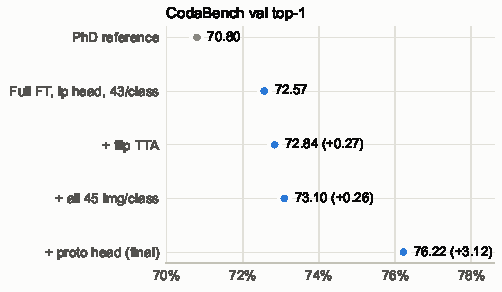
\includegraphics[width=\linewidth]{figures/fig1_codabench_progression_col.pdf}
  \caption{\textbf{CodaBench validation accuracy as we change one setting at a time} (all runs: full fine-tuning, 8 epochs). The gray dot is the reference. Positions encode values, so the axis starts at 70\%.}
  \label{fig:progression}
\end{figure}

\Cref{tab:main} reports all four required metrics for the key models.
Our final full fine-tuning model reaches \textbf{76.22\%} on the CodaBench validation set, 5.4 points above the reference.
It uses 1.03 GPU-hours, 18.9\,GB of memory and the unchanged ViT-B/16 architecture.
\Cref{fig:progression} shows how we got there, one change at a time:
\begin{itemize}[leftmargin=*,itemsep=0pt,topsep=2pt]
    \item flip TTA adds 0.27 points; it changes 4.6\% of the predictions and doubles latency;
    \item training on all 45 images per class adds 0.26 points, which is at the edge of the noise but in the expected direction;
    \item replacing the LP head by the prototype head adds \textbf{3.12 points}.
\end{itemize}
Our final PEFT model, LoRA on all linear layers with a prototype head, reaches \textbf{71.90\%} (+3.6 over the reference LoRA).
It trains 1.375\% of the backbone, and after merging it has exactly the latency of the base model.
Under identical settings (3 epochs, prototype head, holdout), it attains 98\% of full fine-tuning accuracy (71.98\% \vs 73.38\%).
\todo{Phase 2: add CodaBench test accuracy of the final models.}

\subsection{Ablation: classifier head initialization}
\label{sec:ablation-head}

\begin{table}[t]
  \centering
  \footnotesize
  \setlength{\tabcolsep}{4pt}
  \begin{tabular}{@{}lcccc@{}}
    \toprule
    Head init & \shortstack{Head\\alone} & \shortstack{LoRA all\\3 ep\\holdout} & \shortstack{Full FT\\3 ep\\holdout} & \shortstack{Full FT\\8 ep, TTA\\val} \\
    \midrule
    Random & chance & 71.95$^*$ & -- & -- \\
    Prototype & 44.0 & \textbf{72.00}$^*$ & \textbf{73.38} & \textbf{76.22} \\
    Linear probe (LP) & 62.1 & 69.45 & 70.88 & 73.10 \\
    \bottomrule
  \end{tabular}
  \caption{\textbf{Head initialization} (top-1, \%). Within each column only the head initialization changes.
  Head alone: accuracy of the initialized head before training. Full FT 8 ep: all 45 images per class, flip TTA, CodaBench validation.
  $^*$RTX PRO 6000; repeating the prototype run on the A100 gives 71.98.}
  \label{tab:head}
\end{table}

\begin{figure*}[t]
  \centering
  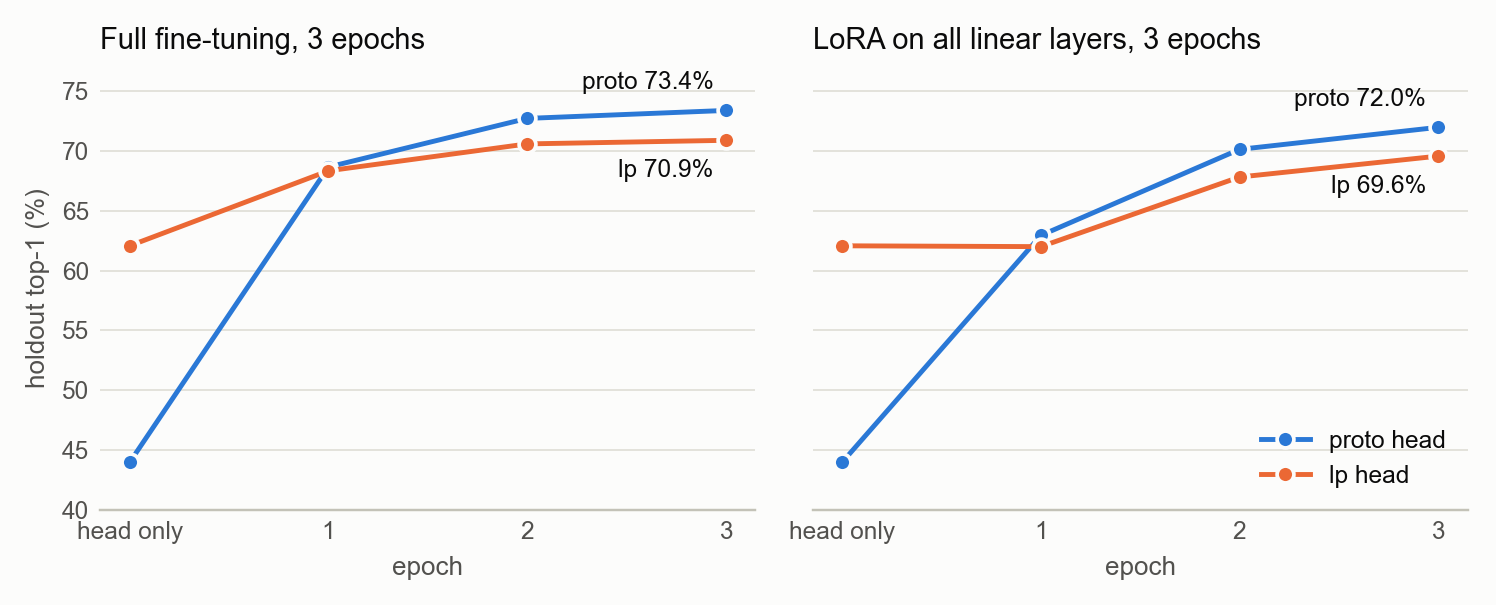
\includegraphics[width=0.92\textwidth]{figures/fig2_head_init_holdout.png}
  \caption{\textbf{Holdout accuracy during training for the LP and prototype heads} (3 epochs; left: full fine-tuning, right: LoRA on all linear layers).
  ``head only'' is the accuracy of the initialized head before any training.
  The LP head starts 18 points higher but finishes about 2.5 points lower.}
  \label{fig:head-curves}
\end{figure*}

\begin{figure*}[t]
  \centering
  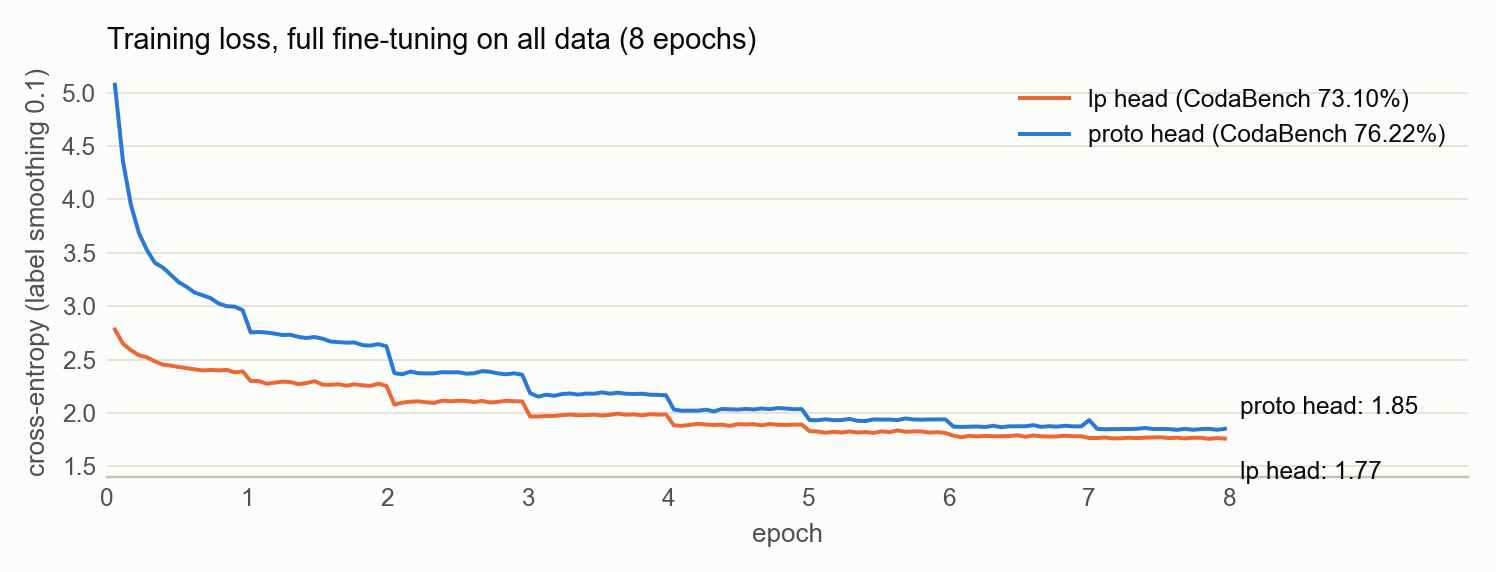
\includegraphics[width=0.92\textwidth]{figures/fig3_loss_lp_vs_proto.png}
  \caption{\textbf{Training loss of full fine-tuning on all data (8 epochs) with the LP and prototype heads}, which differ only in head initialization.
  The prototype model keeps a \emph{higher} training loss (1.85 \vs 1.77 in the last epoch) but scores 3.12 points higher on the validation set.
  The loss drops at every epoch boundary and stays flat within an epoch, a sign that the model is memorizing the 45 images per class.}
  \label{fig:loss}
\end{figure*}

\Cref{tab:head} isolates the head initialization in three settings.
In all three, the LP head is clearly worst, 2.5--3.1 points below the prototype head.
Random and prototype initialization end up level for LoRA (71.95\% \vs 72.00\%).
The prototype head, however, learns faster: it leads by 5 points after the first epoch (63.3\% \vs 58.4\%).
\Cref{fig:head-curves} shows the paradox: the LP head is 18 points better before training and worse after it.

We attribute the LP penalty to the probe having been fitted on \emph{the same images that are then used for fine-tuning}.
The probe already fits them well.
Averaged over the first 100 steps of the LoRA runs, the training loss is 2.29 with the LP head, compared with 4.39 with the prototype head and 9.28 with a random head.
The fine-tuning gradient reaching the backbone is therefore small and dominated by the few examples the probe gets wrong.
Once the features start to move, the fitted head no longer matches them: in the LoRA run with the LP head, the training loss \emph{rises} from 2.22 to 2.69 during the first epoch, before any image has been seen twice.
\Cref{fig:loss} points the same way.
With identical full fine-tuning settings, the LP model reaches a lower training loss but a much lower validation accuracy, \ie, it memorizes more and generalizes less.
A prototype head encodes the class structure, which explains its faster start, without having been fitted to individual training images.
This complements LP-FT~\cite{kumar2022lpft}, which motivates the probe as protection against feature distortion: when the probe is fitted on the fine-tuning images themselves, with only 43--45 images per class, it becomes a liability.

\subsection{Ablation: where to put PEFT capacity}
\label{sec:ablation-peft}

\begin{table}[t]
  \centering
  \footnotesize
  \setlength{\tabcolsep}{3pt}
  \begin{tabular}{@{}lrrrrr@{}}
    \toprule
    LP head, 3 epochs & Params & Holdout & img/s & GB & ms \\
    \midrule
    LoRA qkv, lr $10^{-3}$ & 0.344\% & 68.57 & 1,341 & 13.5 & 7.22 \\
    LoRA qkv, lr $5{\times}10^{-4}$ & 0.344\% & 68.45 & 1,353 & 13.5 & 7.15 \\
    LoRA all linear & 1.375\% & \textbf{69.45} & 885 & 19.9 & 7.03 \\
    AdaptFormer & 1.387\% & 69.05 & 1,437 & 12.8 & 9.89 \\
    \midrule
    Full fine-tuning & 100\% & 70.88 & 1,131 & 18.9 & 7.31 \\
    \bottomrule
  \end{tabular}
  \caption{\textbf{PEFT design.} Params: trainable backbone parameters (head excluded). img/s: training throughput; GB: peak training memory; ms: batch-1 latency after merging (A100, bf16).}
  \label{tab:peft}
\end{table}

\Cref{tab:peft} compares PEFT variants with the LP head for 3 epochs.
\textbf{Capacity matters more than the learning rate.}
Halving the LoRA learning rate changes nothing (\minus0.12, within noise).
Extending LoRA from \texttt{qkv} to all four linear layers, so that the MLP is also adapted, adds 0.88 points while staying far below the 5\% budget for trainable parameters.
\textbf{Mergeable updates matter for deployment.}
AdaptFormer is close in accuracy, but its parallel branches cannot be merged and raise batch-1 latency from about 7.3\,ms to 9.89\,ms ($+$35\%).
\textbf{PEFT does not imply cheaper training here.}
LoRA on all linear layers trains \emph{slower} than full fine-tuning (885 \vs 1,131 img/s) and peaks slightly higher in memory (19.9 \vs 18.9\,GB).
This is presumably because of the 96 extra small, unfused matrix multiplications per forward pass and the activations they keep for the backward pass.
Its savings are in trainable parameters, optimizer state and checkpoint size (35.5\,MB, of which 30.8\,MB is the head, \vs 374\,MB).

\subsection{Ablation: training length}
\label{sec:ablation-length}

\begin{table}[t]
  \centering
  \footnotesize
  \setlength{\tabcolsep}{3.5pt}
  \begin{tabular}{@{}lrrr@{}}
    \toprule
    Setting & Short (ep) & Long (ep) & $\Delta$ \\
    \midrule
    Full FT, LP & 70.88 (3) & 72.31 (8) & $+$1.43 \\
    Full FT, prototype, final$^\ddagger$ & 74.01 (3) & 76.22 (8) & $+$2.21 \\
    LoRA qkv, LP$^\dagger$ & 68.57 (3) & 68.69 (10) & $+$0.12 \\
    LoRA all, LP & 69.45 (3) & 69.87 (6) & $+$0.42 \\
    LoRA all, prototype & 71.98 (3) & 71.52 (6) & \minus0.46 \\
    \bottomrule
  \end{tabular}
  \caption{\textbf{Training length} (holdout top-1, \%; LoRA all: LoRA on all linear layers).
  $^\ddagger$All 45 images per class with flip TTA, CodaBench validation.
  $^\dagger$The 10-epoch run also lowered the head learning rate to $2{\times}10^{-4}$.}
  \label{tab:length}
\end{table}

The two adaptation styles spend the budget very differently (\cref{tab:length}).
Full fine-tuning keeps improving with longer schedules: going from 3 to 8 epochs adds 2.21 points for the final recipe.
LoRA, in contrast, saturates after about 3 epochs, and with the prototype head 6 epochs are worse than 3.
A plausible explanation is the learning rate.
Full fine-tuning uses a small learning rate ($10^{-4}$) that is further reduced for early layers, while LoRA uses $10^{-3}$.
With only 43 images per class, the longer high-learning-rate phase mainly increases memorization.
Its training loss falls much further in 6 epochs (1.70) than in 3 (1.95), while holdout accuracy falls too.
Hence our final PEFT model uses 3 epochs (0.54 GPU-hours) and our final full fine-tuning model uses 8 epochs (1.03 GPU-hours), both within the 1.2-hour budget.

\section{Conclusion}
\label{sec:conclusion}

We adapted ViT-B/16 to a 10,000-class fine-grained benchmark with 45 images per class within a budget of 96\,GB$\cdot$h per run.
The largest gain came from the least glamorous component.
Initializing the 10,000-way head with imprinted class prototypes instead of a linear probe fitted on the training features improved accuracy by 2.5--3.1 points, for both full fine-tuning and LoRA.
With this head, full fine-tuning reaches 76.22\% on the CodaBench validation set in 1.03 GPU-hours.
LoRA on all linear layers reaches 71.90\% while training 1.375\% of the backbone.
After merging, LoRA has zero inference overhead.
For PEFT under this budget, three choices mattered:
\begin{itemize}[leftmargin=*,itemsep=0pt,topsep=2pt]
    \item where the adaptation capacity goes (all linear layers, not only attention);
    \item whether the update can be merged (LoRA \vs AdaptFormer);
    \item a short schedule (about 3 epochs).
\end{itemize}

\paragraph{Limitations.}
Every configuration was trained once (seed 0), and the holdout split has a noise level of about $\pm$0.3 points, so small differences such as the 0.26-point gain from the two extra images per class should be read with care.
The dataset is anonymized, so we cannot relate our findings to its domain.
One ablation batch ran on a different GPU; its accuracies are comparable, as checked by repeating one run, but its speeds and latencies are not.
Our explanation of why the linear-probe head hurts is consistent with the loss curves but is not a controlled proof.
We did not explore higher input resolution, other PEFT families such as VPT or BitFit, or larger budgets.
\todo{Phase 2: report the CodaBench test accuracy of the final models.}
\todo{Check the course page limit (the CVPR limit is 8 pages excluding references).}

{
    \small
    \bibliographystyle{ieeenat_fullname}
    \bibliography{refs}
}

% Appendix: training-log excerpts, full run list and hyperparameters
% Appendix: training-log excerpts, full run list and hyperparameters (generated from the run outputs)
\clearpage
\onecolumn
\appendix

\section{Training-log excerpts}
\label{sec:logs}

The project asks for the training time and VRAM to be documented with training logs.
Below are excerpts of \texttt{train\_log.txt} for our two final models; the full logs (every 100 steps) are available on request.
Dates are removed from the timestamps, Google Drive paths are shortened, and long lines are wrapped.
GPU-hours include head initialization (feature extraction), training and per-epoch holdout evaluation (\cref{sec:budget}).

\paragraph{Final full fine-tuning model} (prototype head, all 45 images per class, 8 epochs, flip TTA at prediction):
{\scriptsize
\begin{verbatim}
========== 1019_1319_1_full ==========
[13:32:14] full: lr 0.0001, head lr 0.0001, wd 0.05, layer decay 0.75, epochs 8, holdout 0/class,
           head init proto, time budget 1.20 h
[13:32:14] Environment: NVIDIA A100-SXM4-80GB (80 GB), bfloat16, 12 CPUs |
           torch 2.11.0+cu130 (CUDA 13.0), timm 1.0.30, peft 0.21.1
[13:38:32] Extracted features for 450,000 train / 0 holdout images in 6.1 min
[13:38:32] Head initialized from proto (6.2 min incl. feature extraction, counted in this run's GPU time)
[13:38:32] Trainable (excl. head): 85,798,656 = 100.000% of backbone | head 7,690,000 params (fine-tuned)
[13:38:32] Training up to 8 epochs x 1757 steps (batch 256x1, warmup 1757 steps)
[13:40:03] Speed 1146 img/s, 6.5 min/epoch
[13:46:13] == epoch 1: train loss 3.4158, 13.8 min used
[13:52:55] == epoch 2: train loss 2.6899, 20.5 min used
[13:59:51] == epoch 3: train loss 2.3729, 27.4 min used
[14:06:42] == epoch 4: train loss 2.1758, 34.2 min used
[14:13:40] == epoch 5: train loss 2.0321, 41.1 min used
[14:20:31] == epoch 6: train loss 1.9367, 47.9 min used
[14:27:32] == epoch 7: train loss 1.8741, 54.9 min used
[14:34:26] == epoch 8: train loss 1.8491, 61.8 min used
[14:34:29] Training done: 14056 steps, 1.03 GPU-hours (budget 1.20 h)
[14:34:29] Peak VRAM: 18.9 GB allocated, 20.1 GB reserved by PyTorch (GPU has 80 GB)
[14:34:32] Inference latency (batch 1): 14.95 ms/img | throughput (batch 256): 1919 img/s |
           NVIDIA A100-SXM4-80GB, bfloat16, with flip TTA
[14:35:29] [val] 50,000 predictions over 9,992 classes (max 13 per class) ->
           .../submission_val_1019_1319_1_full.zip
\end{verbatim}
}

\paragraph{Final PEFT model} (LoRA on all linear layers, prototype head, 3 epochs, 2 images per class held out):
{\scriptsize
\begin{verbatim}
========== 1019_1319_3_lora ==========
[14:57:51] lora: lr 0.001, head lr 0.001, wd 0.0001, layer decay 1.0, epochs 3, holdout 2/class, head init proto,
           time budget 1.20 h
[14:57:51] Environment: NVIDIA A100-SXM4-80GB (80 GB), bfloat16, 12 CPUs |
           torch 2.11.0+cu130 (CUDA 13.0), timm 1.0.30, peft 0.21.1
[15:06:07] Extracted features for 430,000 train / 20,000 holdout images in 7.2 min
[15:06:08] Prototype head (zero-shot, 0 trainable params): holdout top-1 44.01%
[15:06:08] Head initialized from proto (7.2 min incl. feature extraction, counted in this run's GPU time)
[15:07:15] Trainable (excl. head): 1,179,648 = 1.375% of backbone | head 7,690,000 params (fine-tuned)
[15:07:15] Training up to 3 epochs x 1679 steps (batch 256x1, warmup 503 steps)
[15:07:53] Speed 888 img/s, 8.1 min/epoch
[15:15:44] == epoch 1: train loss 3.2174, holdout top-1 62.94%, 15.7 min used
[15:24:12] == epoch 2: train loss 2.4125, holdout top-1 70.12%, 24.2 min used
[15:32:40] == epoch 3: train loss 1.9496, holdout top-1 71.97%, 32.6 min used
[15:32:41] Training done: 5037 steps, 0.54 GPU-hours (budget 1.20 h)
[15:32:41] Peak VRAM: 19.9 GB allocated, 21.3 GB reserved by PyTorch (GPU has 80 GB)
[15:33:00] Final holdout: top-1 71.98%, top-5 89.07%
[15:33:03] Inference latency (batch 1): 7.61 ms/img | throughput (batch 256): 3869 img/s |
           NVIDIA A100-SXM4-80GB, bfloat16, no flip TTA
[15:33:55] [val] 50,000 predictions over 9,991 classes (max 15 per class) ->
           .../submission_val_1019_1319_3_lora.zip
\end{verbatim}
}

\section{All runs}
\label{sec:all-runs}

\begin{table}[h]
  \centering
  \footnotesize
  \setlength{\tabcolsep}{3pt}
  \begin{tabular}{@{}lllrrrrrrr@{}}
    \toprule
    Run & Method & Head & Ep. & Trainable & Holdout & Val & GPU-h & GB & ms \\
    \midrule
    \run{0928\_0636\_1\_linear} & Zero-shot & prototype & 0 & 0 & 43.95 & -- & 0.11 & 3.9 & 7.55 \\
    \run{0928\_0636\_3\_full} & Full FT & LP & 3 & 100\% & 70.88 & -- & 0.45 & 18.9 & 7.31 \\
    \run{0928\_0748\_1\_full} & Full FT & LP & 8 & 100\% & 72.31 & 72.57/72.84$^\ddagger$ & 1.03 & 18.9 & 7.35 \\
    \run{1018\_2306\_1\_full} & Full FT, all data & LP & 8 & 100\% & -- & 73.10$^\ddagger$ & 1.03 & 18.9 & 14.92$^\ddagger$ \\
    \run{1019\_1120\_1\_full} & Full FT & prototype & 3 & 100\% & 73.38 & -- & 0.48 & 18.9 & 7.78 \\
    \run{1019\_1319\_2\_full} & Full FT, all data & prototype & 3 & 100\% & -- & 74.01$^\ddagger$ & 0.44 & 18.9 & 15.24$^\ddagger$ \\
    \run{1019\_1319\_1\_full} & \textbf{Full FT, all data (final)} & prototype & 8 & 100\% & -- & \textbf{76.22}$^\ddagger$ & 1.03 & 18.9 & 14.95$^\ddagger$ \\
    \midrule
    \run{0928\_0636\_2\_lora} & LoRA qkv & LP & 3 & 0.344\% & 68.57 & -- & 0.40 & 13.5 & 7.22 \\
    \run{0928\_0748\_2\_lora} & LoRA qkv, head lr $2{\times}10^{-4}$ & LP & 10 & 0.344\% & 68.69 & -- & 1.06 & 13.5 & 7.53 \\
    \run{1018\_1239\_1\_lora} & LoRA qkv, lr $5{\times}10^{-4}$ & LP & 3 & 0.344\% & 68.45 & -- & 0.41 & 13.5 & 7.15 \\
    \run{1018\_1239\_3\_adaptformer} & AdaptFormer & LP & 3 & 1.387\% & 69.05 & -- & 0.39 & 12.8 & 9.89 \\
    \run{1018\_1239\_2\_lora} & LoRA all & LP & 3 & 1.375\% & 69.45 & -- & 0.55 & 19.9 & 7.03 \\
    \run{1018\_2306\_2\_lora} & LoRA all & LP & 6 & 1.375\% & 69.87 & -- & 0.97 & 19.9 & 7.31 \\
    \run{1019\_0953\_1\_lora}$^*$ & LoRA all & random & 3 & 1.375\% & 71.95 & -- & 0.37$^*$ & 19.9 & 1.81$^*$ \\
    \run{1019\_0953\_2\_lora}$^*$ & LoRA all & prototype & 3 & 1.375\% & 72.00 & -- & 0.44$^*$ & 19.9 & 1.82$^*$ \\
    \run{1019\_1120\_2\_lora} & LoRA all & prototype & 6 & 1.375\% & 71.52 & -- & 0.97 & 19.9 & 7.76 \\
    \run{1019\_1319\_3\_lora} & \textbf{LoRA all (final PEFT)} & prototype & 3 & 1.375\% & \textbf{71.98} & \textbf{71.90} & 0.54 & 19.9 & 7.61 \\
    \bottomrule
  \end{tabular}
  \caption{\textbf{All 17 runs.} Run IDs encode the batch start time (month, day, hour, minute) and the position in the batch.
  LoRA all: LoRA on all linear layers. Trainable: backbone parameters excluding the 7.69M head. GB: peak allocated memory during training. ms: batch-1 latency.
  $^\ddagger$Predicted with flip TTA. $^*$Run on an RTX PRO 6000 Blackwell; all other runs on an A100-SXM4-80GB (speed and latency are not comparable across the two).
  The linear-probe head (62.07\% holdout) is computed inside every LP run and has no separate run.}
  \label{tab:all-runs}
\end{table}

\section{Hyperparameters}
\label{sec:hparams}

\begin{table}[h]
  \centering
  \footnotesize
  \renewcommand{\arraystretch}{1.15}
  \begin{tabular}{@{}p{2.2cm}p{3.5cm}p{3.5cm}p{3.5cm}p{3.0cm}@{}}
    \toprule
    & Full fine-tuning & LoRA & AdaptFormer & Linear-probe head \\
    \midrule
    Trainable & all weights + head & $A, B$ in qkv, proj, fc1, fc2 (all 12 blocks) + head & parallel MLP adapters + head & head only, on cached features \\
    Method-specific & layer-wise lr decay 0.75, drop path 0.1 & $r=8$, $\alpha=16$, no dropout, merged after training & bottleneck 64, scale 0.1, dropout 0.1 & initialized from the prototype head \\
    Optimizer & AdamW & AdamW & AdamW & AdamW \\
    Learning rate & $10^{-4}$ (head $10^{-4}$) & $10^{-3}$ (head $10^{-3}$) & $10^{-3}$ (head $10^{-3}$) & $10^{-3}$ \\
    Weight decay & 0.05 & $10^{-4}$ & $10^{-4}$ & $10^{-4}$ \\
    Schedule & \multicolumn{3}{p{11.3cm}}{linear warmup (1 epoch; 0.3 epochs for 3-epoch runs), then cosine decay to 0} & cosine, no warmup \\
    Epochs & 3 or 8 & 3, 6 or 10 & 3 & 10 \\
    Batch size & 256 & 256 & 256 & 4,096 \\
    Precision & bf16 & bf16 & bf16 & fp32 head, fp16 features \\
    Regularization & \multicolumn{3}{p{11.3cm}}{label smoothing 0.1, gradient clipping at norm 1.0} & label smoothing 0.1 \\
    Augmentation & \multicolumn{3}{p{11.3cm}}{RandomResizedCrop (scale 0.25--1) + horizontal flip} & none (center crops) \\
    \bottomrule
  \end{tabular}
  \caption{\textbf{Hyperparameters.} Weight decay is not applied to biases, normalization parameters, the class token and position embeddings. Evaluation resizes to 248 pixels and takes a 224 center crop.}
  \label{tab:hparams}
\end{table}


\end{document}
